\documentclass[handout]{beamer}
%\documentclass [serif,mathserif,professionalfont]{beamer} 
%\usepackage {pxfonts}
%\usepackage {eulervm}
%\usepackage{mathpazo}
%\logo{\includegraphics[height=1.2cm]{fsulogo.png}}

\usepackage{tikz}
\usepackage{graphicx}
\usepackage{multimedia}
\usepackage[latin1]{inputenc}
%\usetheme{Warsaw}
\usecolortheme{lily}
\setbeamercovered{transparent}
%\useoutertheme[subsection=false]{smoothbars}

\title[EVA, Ann Arbor, MI 2015 \insertdate]{Examples of extreme event modeling in\\ tornado and hurricane research}

\author{James B. Elsner\\ Twitter: \alert{@JBElsner}}
\institute{Florida State University, Tallahassee, FL}
\date{June 15, 2015}

\begin{document}

\begin{frame}
\titlepage
Help: Thomas H. Jagger
\end{frame}

\section{Are Tornadoes More Likely Over Smooth Terrain?}

\begin{frame}
\begin{center}
{\Large Are Tornadoes More Likely Over Smooth Terrain?}\\
\vspace{.5cm}
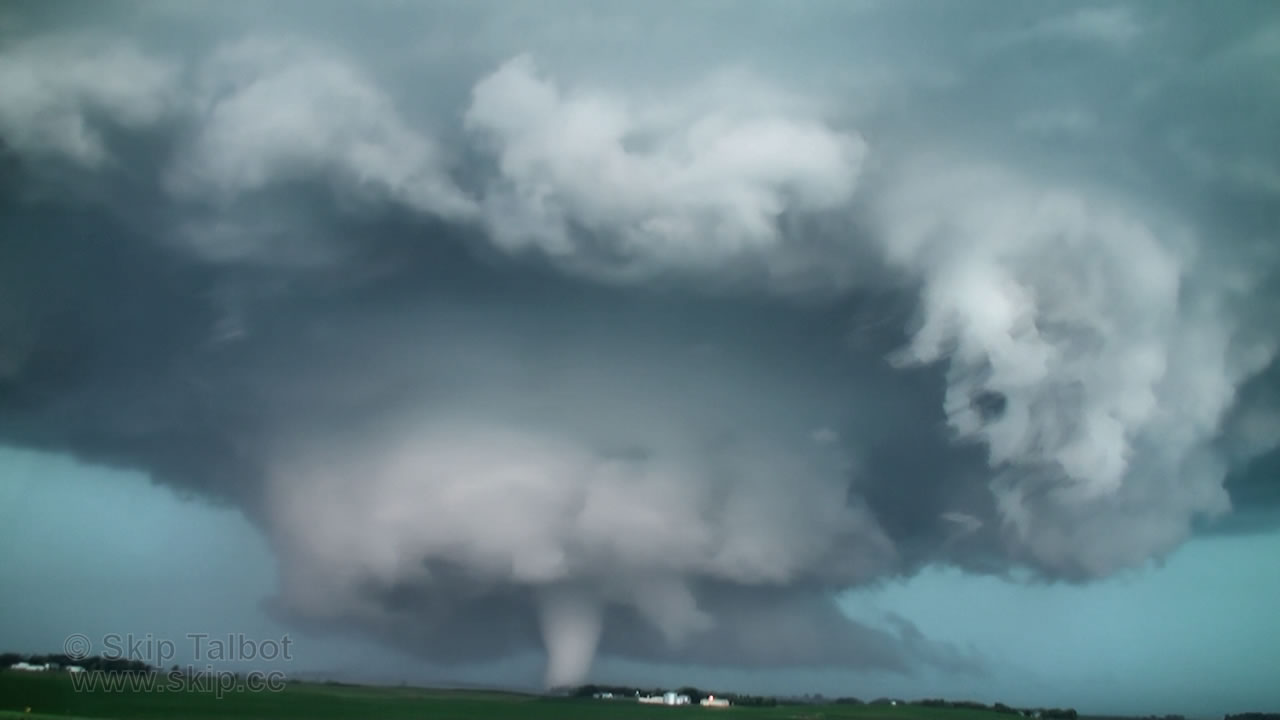
\includegraphics[scale = .25]{figures/TornMeso2.jpg}
\end{center}
\end{frame}

\begin{frame}{Problem: Tornado reports are not tornadoes}
\begin{itemize}
\item How can we extract information about tornadoes from the limited tornado reports?
\item There are more tornado reports near cities and towns, but it's unlikely that cities are causing tornadoes.
\end{itemize}
\begin{columns}
\begin{column}{6cm}
\begin{itemize}
\item We need to control for non-weather influences if we want to understand what factors cause more tornadoes in certain regions.
\item For instance, we suggest terrain roughness will disrupt the flow of air into the meso-cyclone making a tornado less likely.
\end{itemize}
\end{column}
\begin{column}{4cm}
\begin{center}
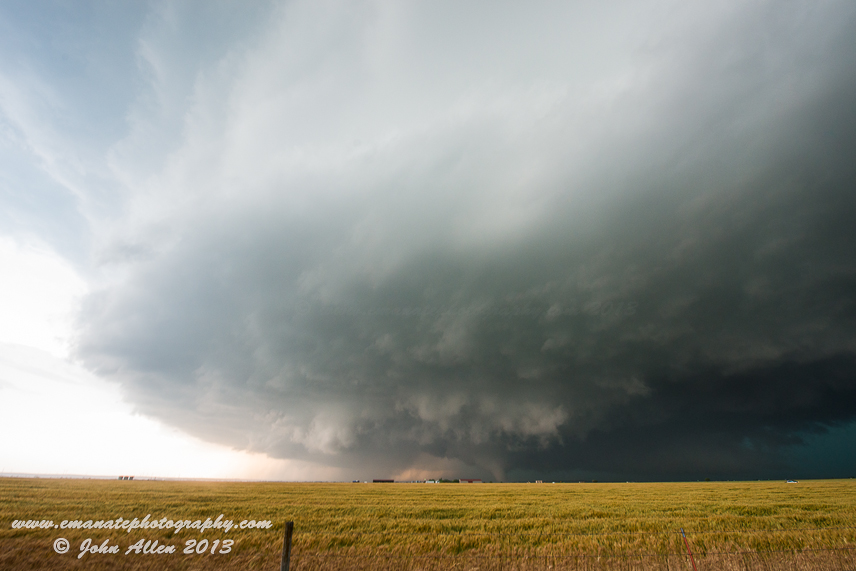
\includegraphics[scale = .32]{figures/TornMeso.jpg}
\end{center}
\end{column}
\end{columns}
\end{frame}

\begin{frame}{If we solve this problem, then this map}
\begin{center}
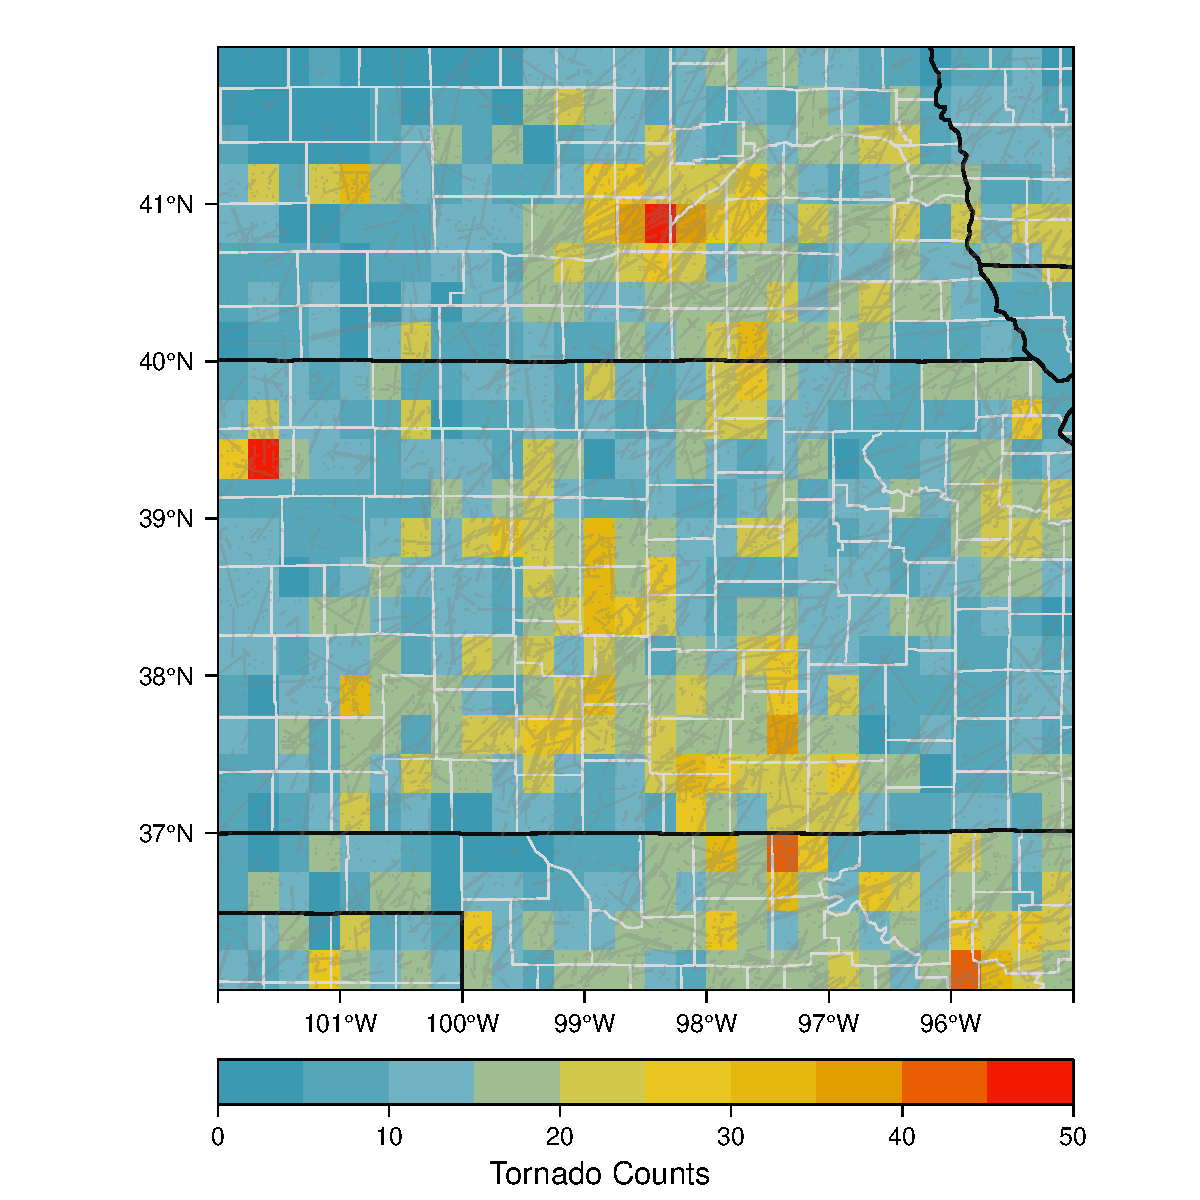
\includegraphics[scale=.41]{figures/PathsGrids.pdf}
\end{center}
\end{frame}

\begin{frame}{Becomes these maps}
\vspace{-1cm}
\begin{center}
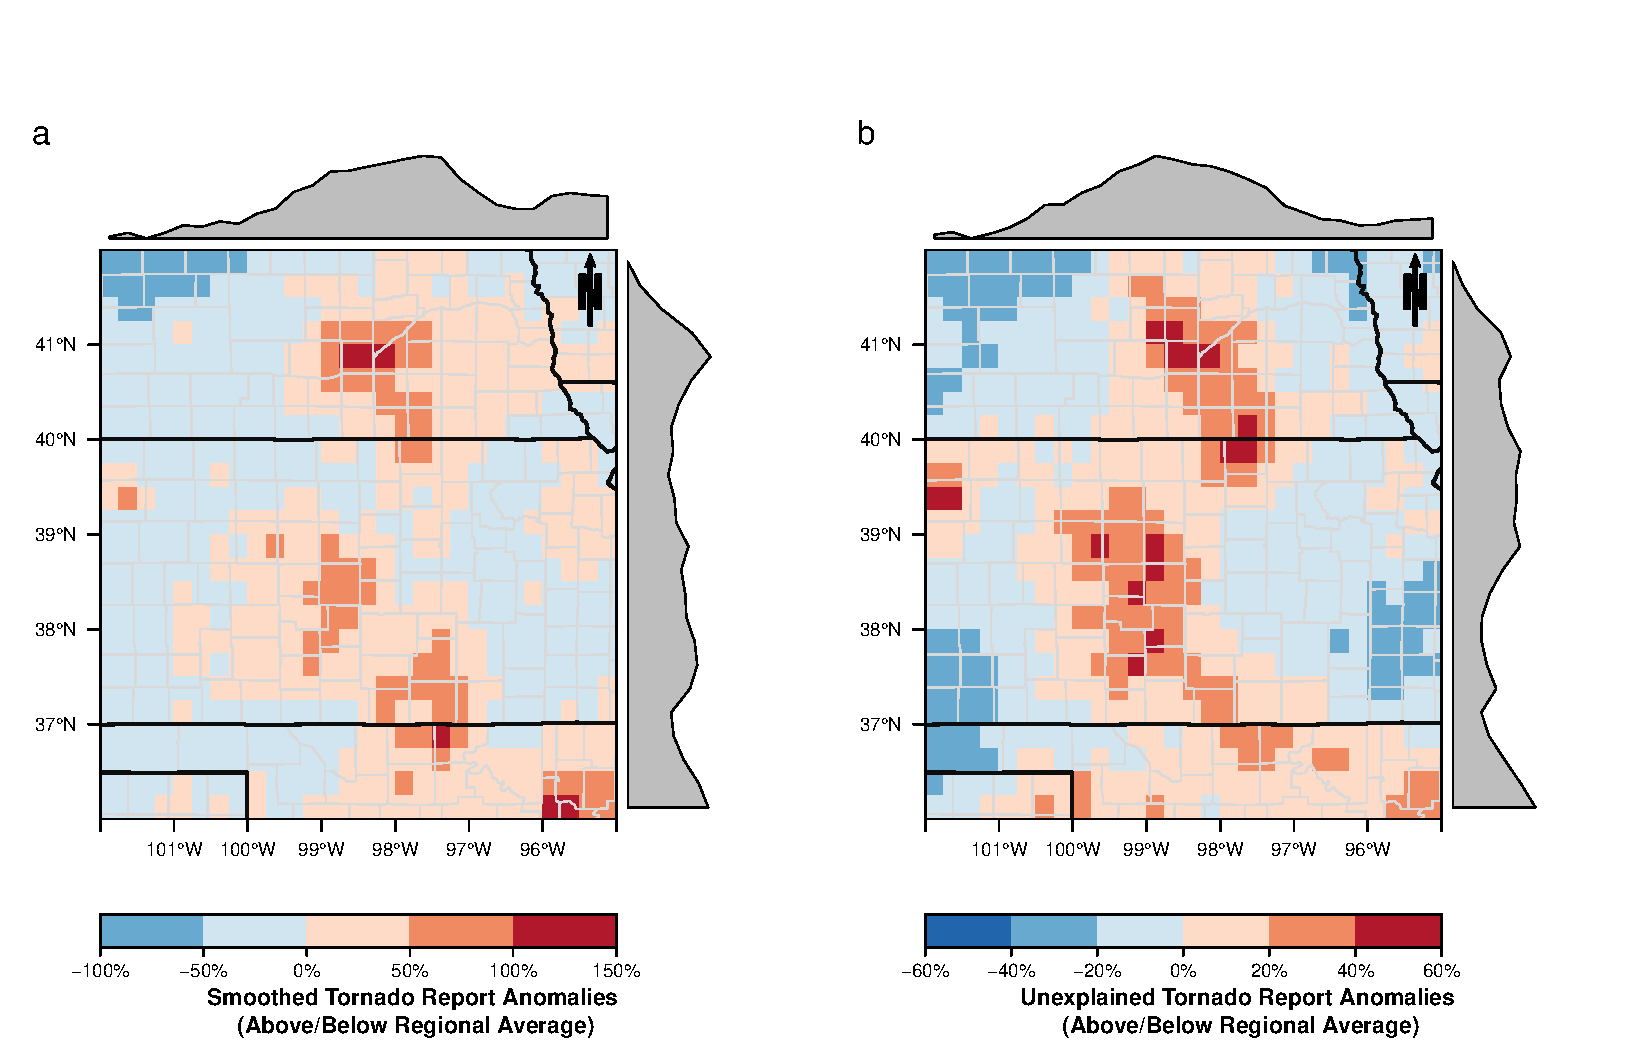
\includegraphics[scale=.42]{figures/TornadoReports.pdf}
\end{center}
\end{frame}

\begin{frame}{Case study}
\vspace{-1cm}
\begin{center}
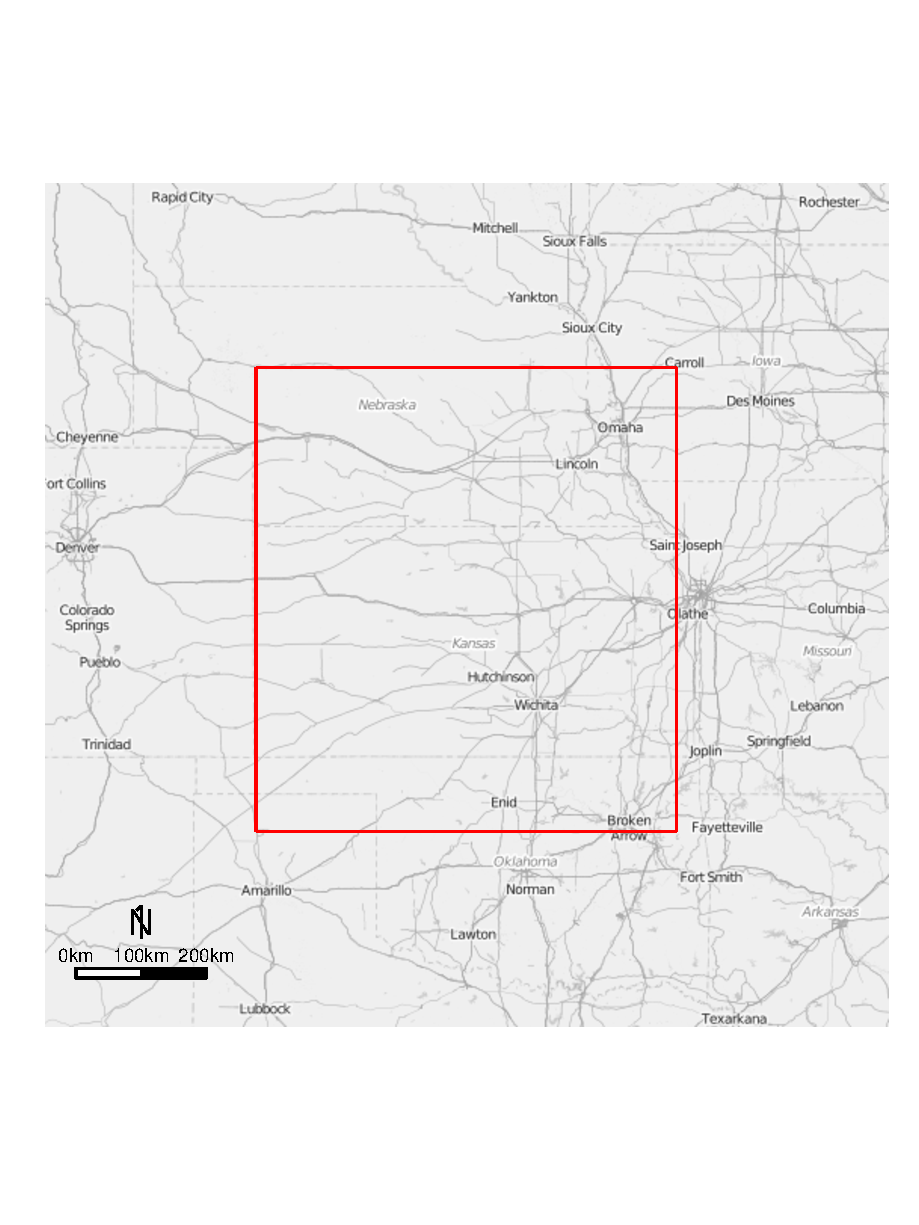
\includegraphics[scale=.48]{figures/DomainMap.pdf}
\end{center}
\end{frame}

\begin{frame}{Population \& terrain roughness variables}
\vspace{-1cm}
\begin{center}
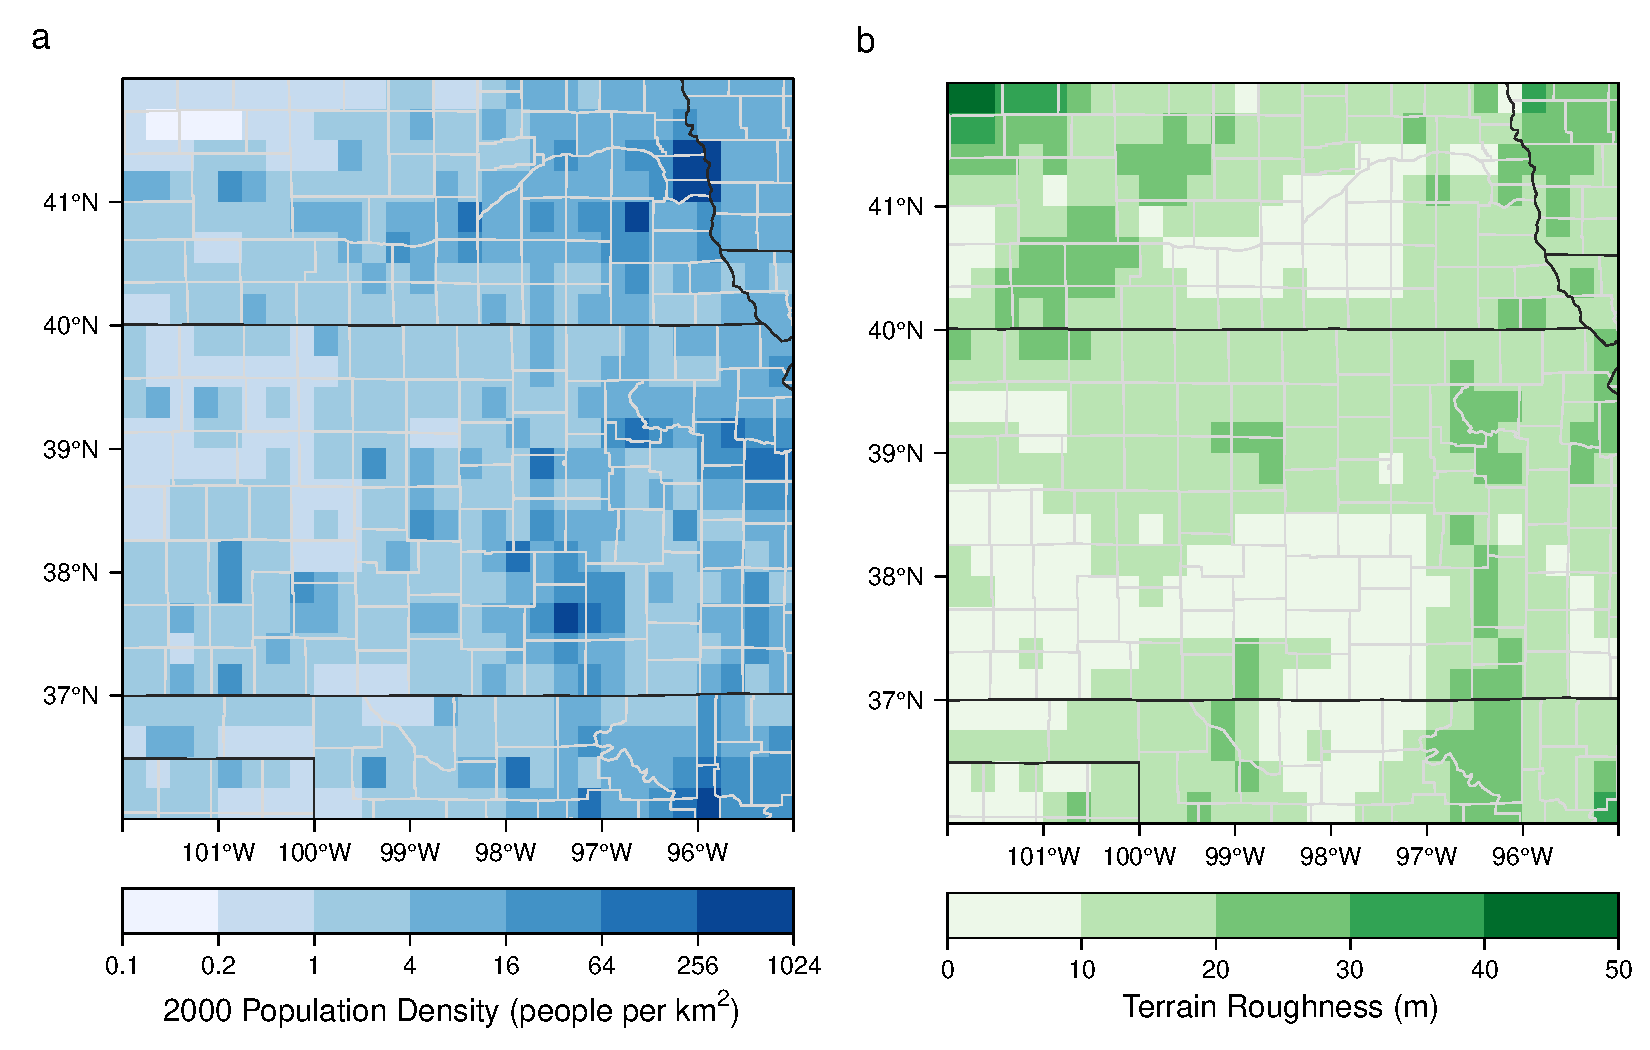
\includegraphics[scale=.4]{figures/PopTRMap.pdf}
\end{center}
\end{frame}

\begin{frame}{Exploratory analysis}
\vspace{-1cm}
\begin{center}
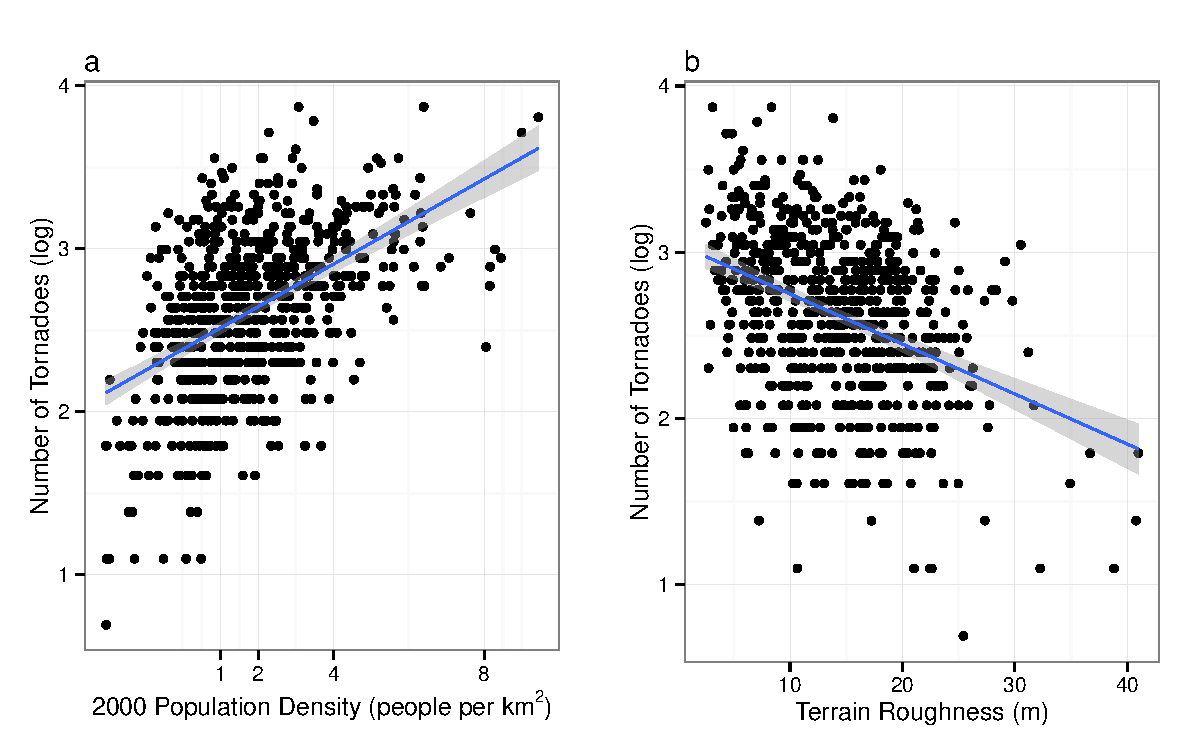
\includegraphics[scale=.54]{figures/Scatterplots.pdf}
\end{center}
\end{frame}

\begin{frame}{Exploratory analysis}
\vspace{-1cm}
\begin{center}
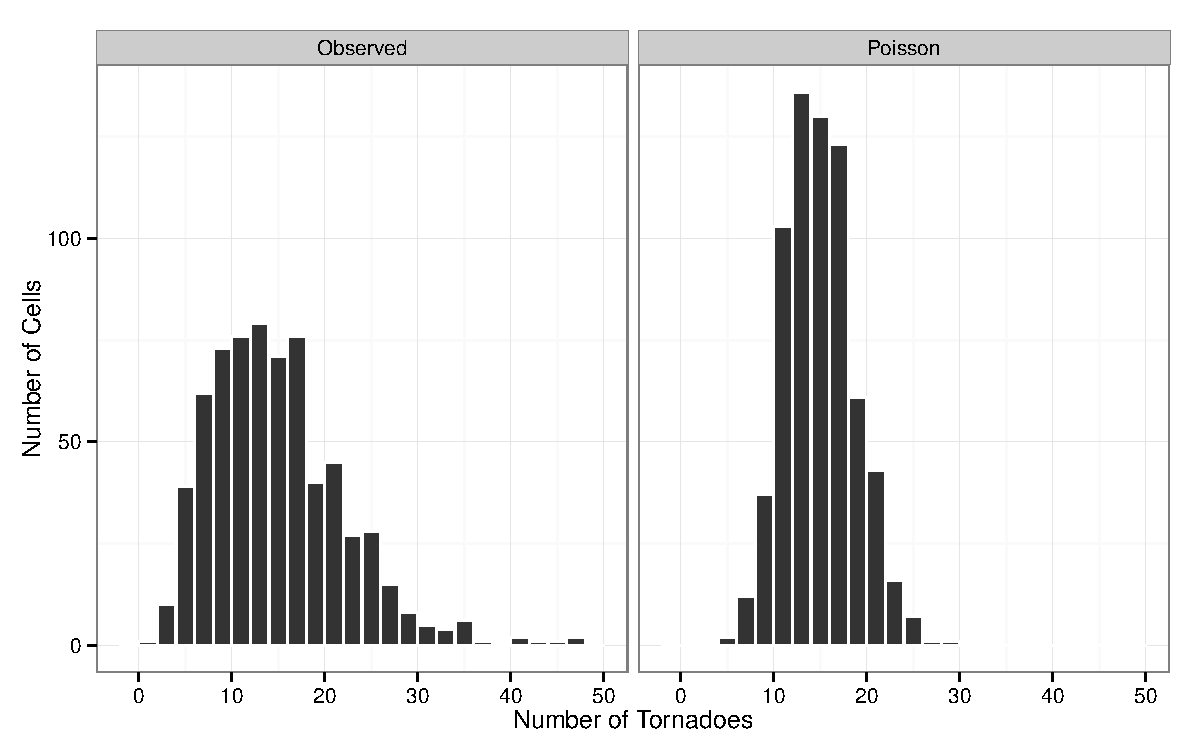
\includegraphics[scale=.54]{figures/Distribution.pdf}
\end{center}
\end{frame}

\begin{frame}{Model}
\begin{eqnarray*}
T_s | \mu_s, n&\sim& \hbox{NegBin}(\mu_s, n)   \\
\mu_s &=& \exp(\nu_s) \cdot \hbox{area}_s \\
\nu_s &=& \beta_0 + \beta_{Pop}\cdot\log_2(\hbox{Pop}_s) + \beta_{TR} \hbox{TR}_s + u_s,
\end{eqnarray*}
where NegBin($\mu_s$, $n$) indicates that the conditional tornado count ($T_s|\mu_s,n$) is described by a negative binomial distribution with mean $\mu_s$ and dispersion $n$. The mean depends on the cell area (exposure) and is linearly related to the fixed and random effects through the logarithmic link function ($\nu_s$). The fixed effects include population density (Pop$_s$) and terrain roughness (TR$_s$).
\end{frame}

\begin{frame}{Spatial autocorrelation}
The random effect ($u_s$) follows a Besag formulation where
$$
u_i | u_j, i \neq j, \tau \sim N\left(\frac{1}{m_i} \sum_{i \sim j} u_j , \frac{1}{m_i} \tau\right)
$$
where $N$ is the normal distribution with mean $1/m_i \cdot \sum_{i \sim j} u_j$ and variance $1/m_i \cdot \tau$ where $m_i$ is the number of neighboring cells and $\tau$ is the precision; $i \sim j$ indicates cells $i$ and $j$ are neighbors.
\end{frame}

\begin{frame}{Fixed effects}
\vspace{-1cm}
\begin{center}
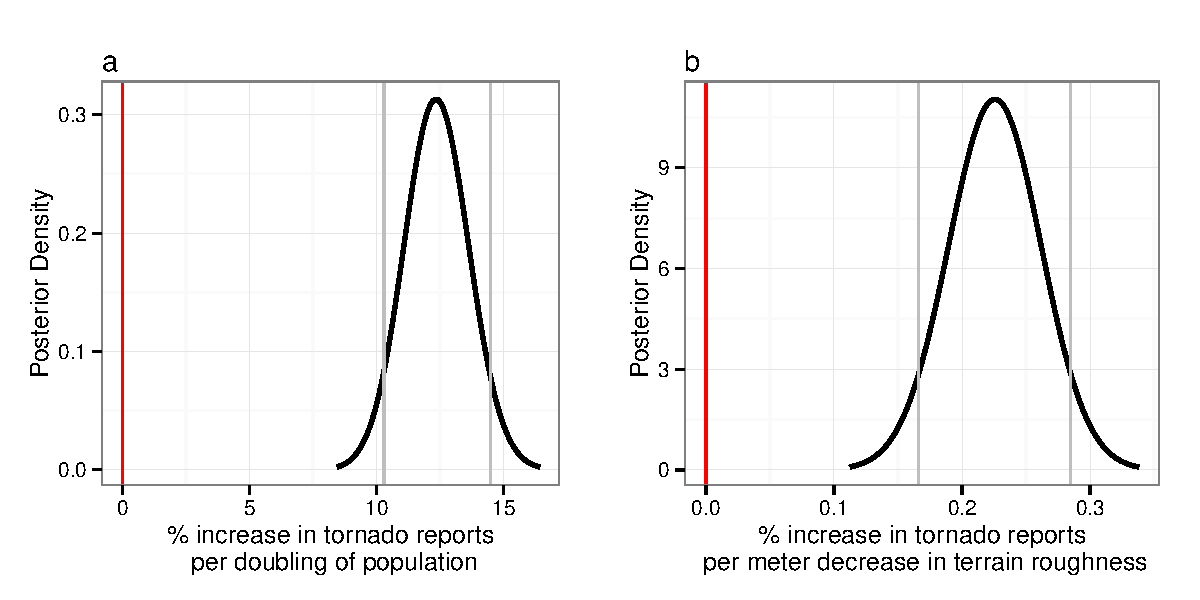
\includegraphics[scale=.54]{figures/FixedEffects.pdf}
\end{center}
\end{frame}

\begin{frame}{Sensitivity}
\begin{small}
\begin{table}
\begin{center}
\caption{Terrain roughness effect in models of tornado activity. The effect has units of \% increase in tornadoes per meter decrease in roughness.}
\begin{tabular}{cccccc} \hline
Start    & EF       & Grid   & Tornado & Terrain Roughness Effect            \\
Year     & Range    & Size   & Reports & (per m decrease in roughness)       \\ \hline
1955  & EF0$+$ & .250$^\circ$  & 6749  & $\underset{(1.5\%, 3.0\%)}{2.2\%}$ \\
\alert{1975}  & EF0$+$ & .250$^\circ$  & 4898  & $\underset{(1.4\%, 3.1\%)}{2.2\%}$ \\
\alert{1995}  & EF0$+$ & .250$^\circ$  & 2940  & $\underset{(1.4\%, 3.6\%)}{2.5\%}$ \\
1955  & \alert{EF1$+$} & .250$^\circ$  & 3054  & $\underset{(1.6\%, 3.4\%)}{2.5\%}$ \\
1955  & \alert{EF2$+$} & .250$^\circ$  & 1159  & $\underset{(1.9\%, 4.4\%)}{3.2\%}$ \\
1955  & \alert{EF3$+$} & .250$^\circ$  &  368  & $\underset{(2.0\%, 5.4\%)}{3.7\%}$ \\
1955  & EF0$+$ & \alert{.125$^\circ$}  & 6749  & $\underset{(1.4\%, 2.6\%)}{2.0\%}$ \\
1955  & EF0$+$ & \alert{.0625$^\circ$} & 6749  & $\underset{(1.3\%, 2.1\%)}{1.7\%}$ \\
\hline
\end{tabular}
\end{center}
\end{table}
\end{small}

\end{frame}

\begin{frame}{Spatial random effect}
\begin{center}
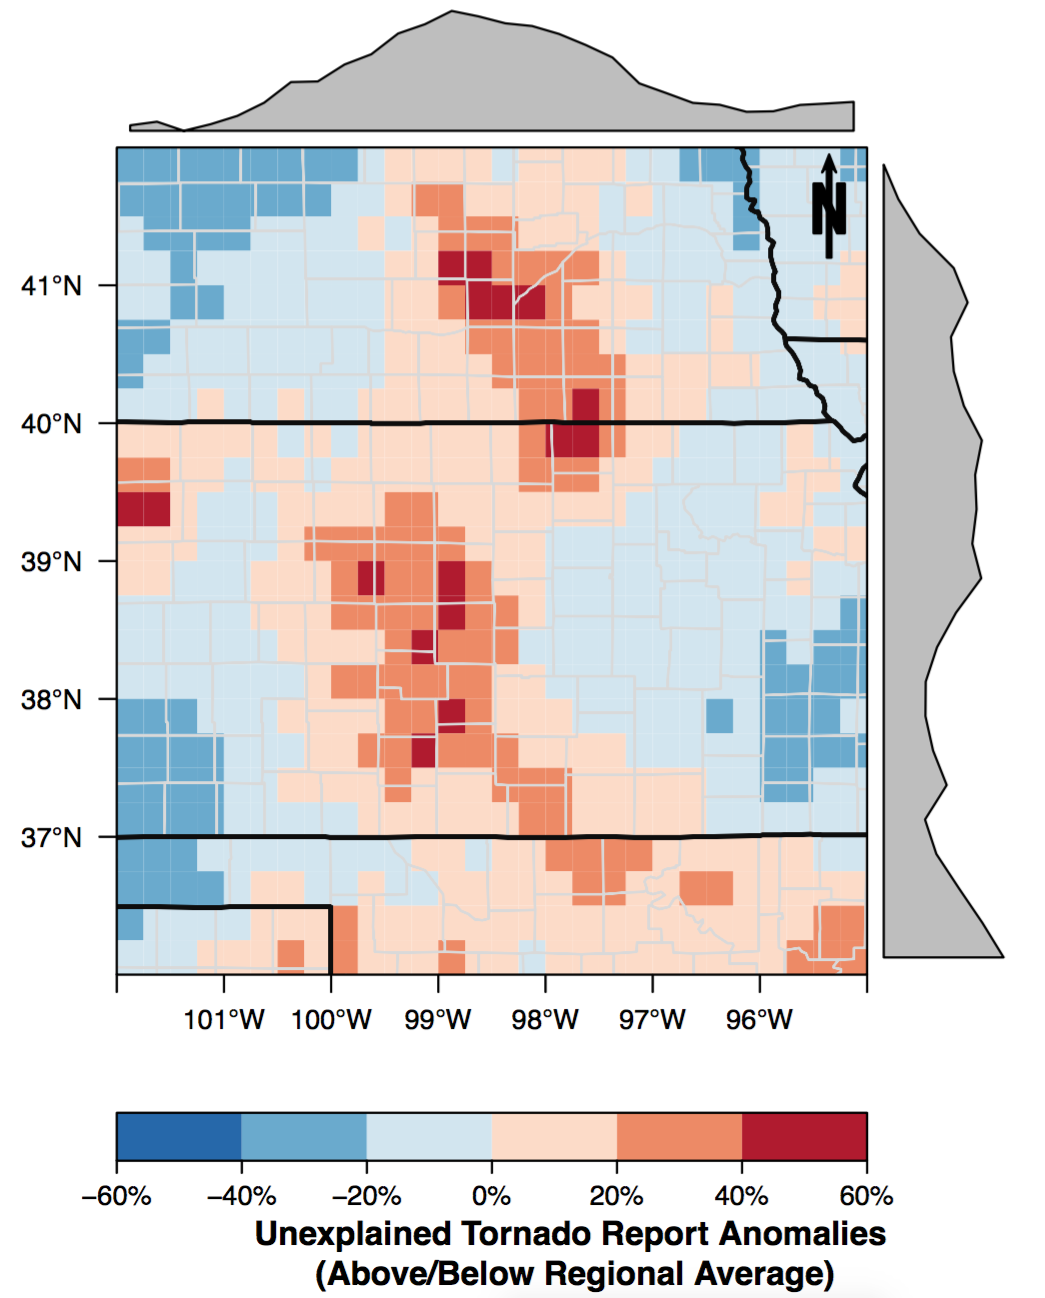
\includegraphics[scale=.18]{figures/Unexplained.png}
\end{center}
\end{frame}

\section{How Sensitive Are Hurricanes to Ocean Heat?}

\begin{frame}
\begin{center}
{\Large How Sensitive Are Hurricanes to Ocean Heat?}\\
\vspace{.5cm}
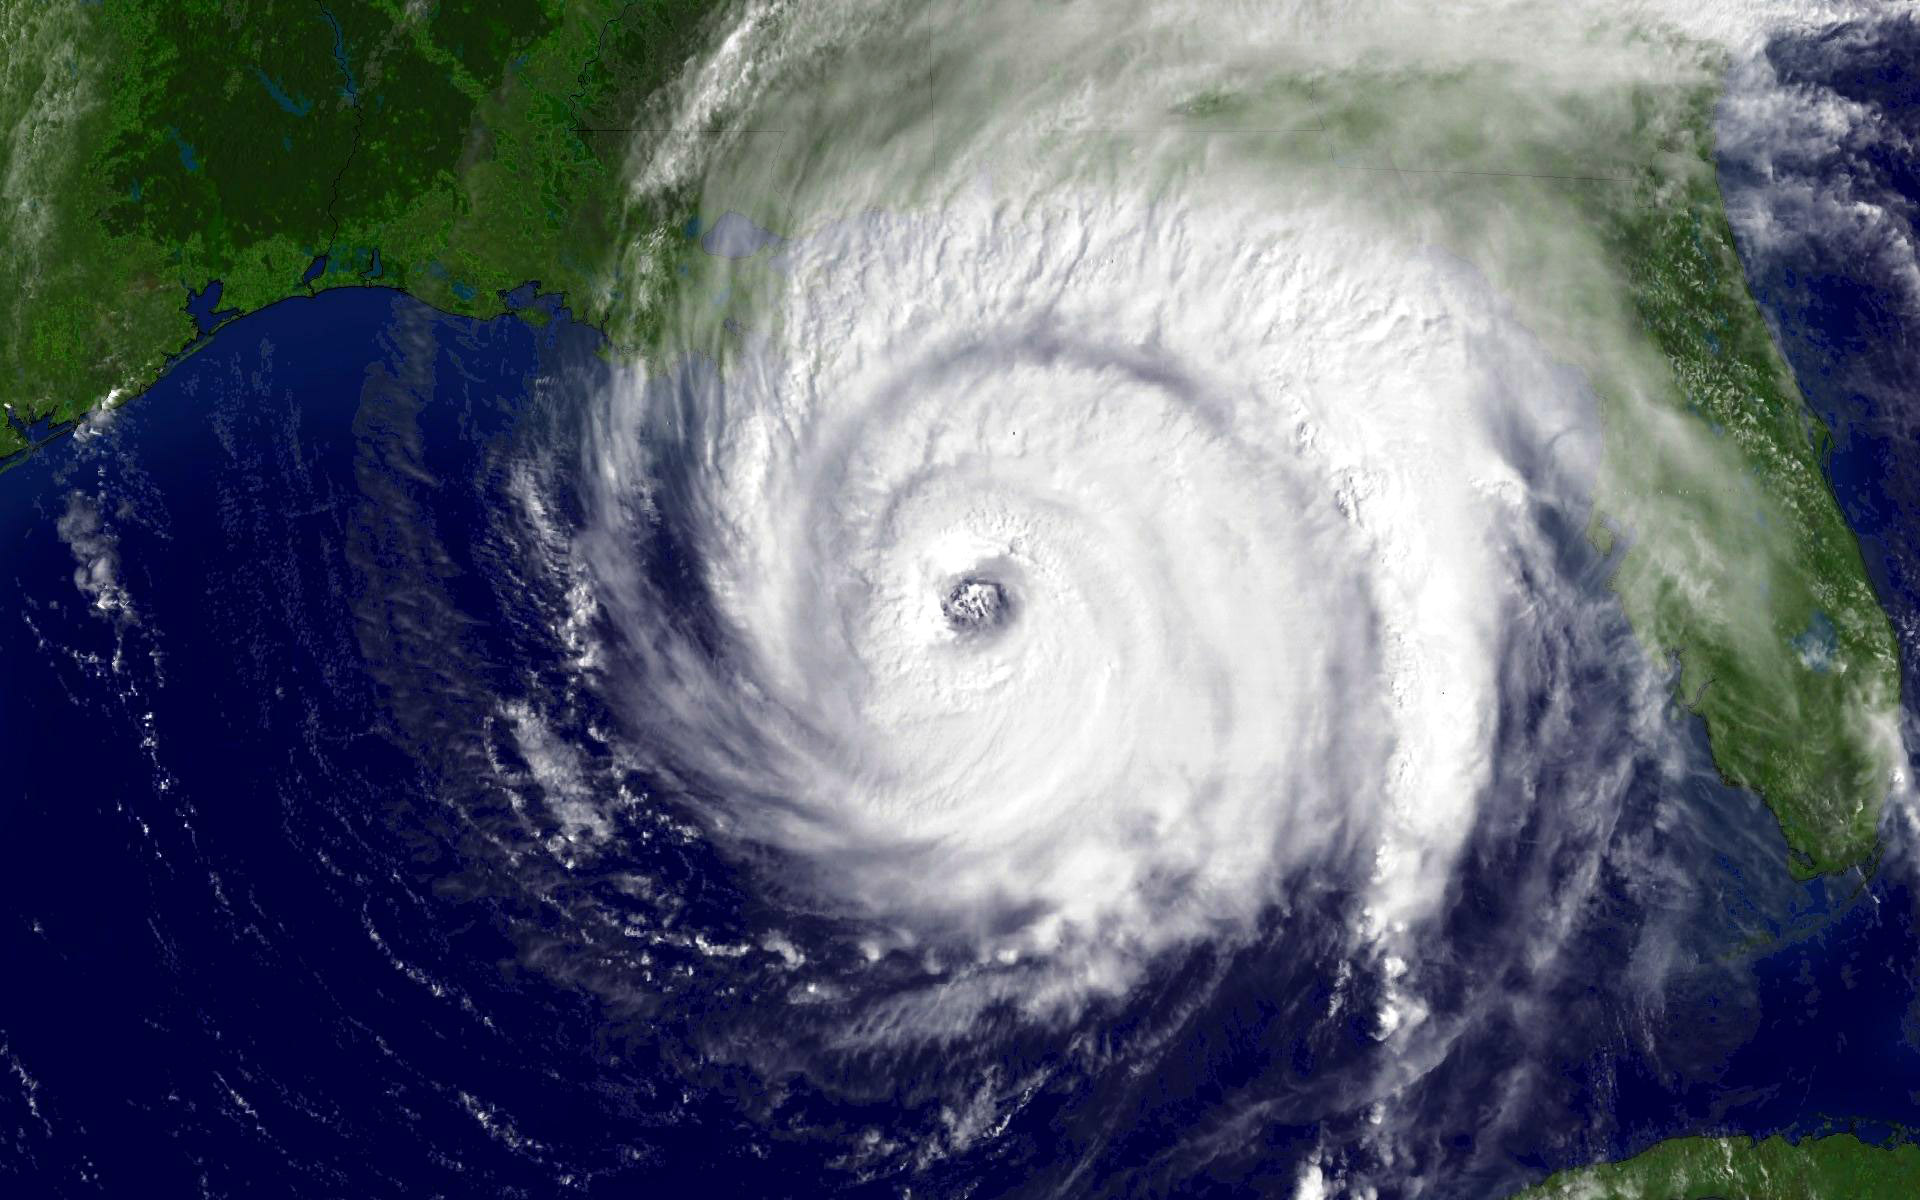
\includegraphics[scale=.14]{figures/ivan091504-1515z.jpg}
\end{center}
{\footnotesize Photo Credit: NOAA}
\end{frame}

\begin{frame}{Problem}
\begin{itemize}
\item We know what hurricanes are like today. When, where, how often. They are sometimes deadly and destructive.  
\item What about tomorrow? Will there be more? Will they be stronger?
\item How do we get answers to these questions?
\end{itemize}

Unfortunately there are no simply ways.
\begin{itemize}
\item \alert{Theory} is limited. We don't have a theory of climate. We don't know all the processes that affect hurricanes.
\item \alert{Models} don't adequately represent the atmosphere or the ocean. And they don't adequately resolve hurricanes.
\item \alert{Data}sets are of limited length and of variable quality. 
\end{itemize}
\end{frame}

\begin{frame}{Solution}
Start with the available theory. Use quality data to estimate a key quantity from the theory. Estimate the same quantity using model data. Make comparisons.
\begin{itemize}
\item Available theory: Hurricanes as heat engines and the statistics of extreme values.
\item Quality data: National Hurricane Center's best-track data with modifications.
\item Models: Global Climate Models from CMIP5 used by the IPCC.
\end{itemize}
\end{frame}

\begin{frame}{Hurricanes as heat engines}
\begin{columns}
\begin{column}{5cm}
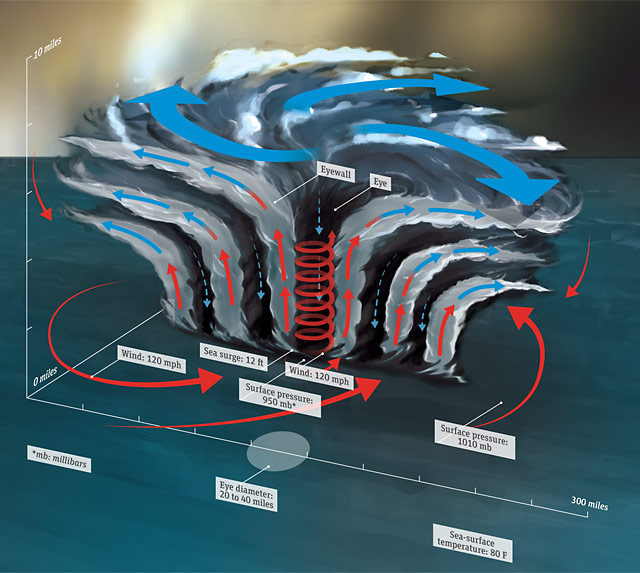
\includegraphics[scale=.2]{figures/heatEngine.jpg}\\
{\footnotesize Photo credit: {\it Popular Mechanics}}
\end{column}
\begin{column}{6cm}
\begin{center}
\alert{Maximum Potential Intensity (MPI) Theory}
\end{center}
$$
\hbox{MPI} \sim \frac{\hbox{SST}}{T_o}\hbox{BL}_{f}(\hbox{SST})
$$
MPI is the highest wind speed (rotational) in units of meters per second. SST is the ocean temperature at the surface, $T_o$ is the temperature at the top of the hurricane and BL$_{f}$(SST) are heat fluxes involving potential temperature of saturated air. The heat fluxes depend on SST.
\end{column}
\end{columns}
\end{frame}

\begin{frame}{Extreme value theory}
\vspace{-1cm}
\begin{center}
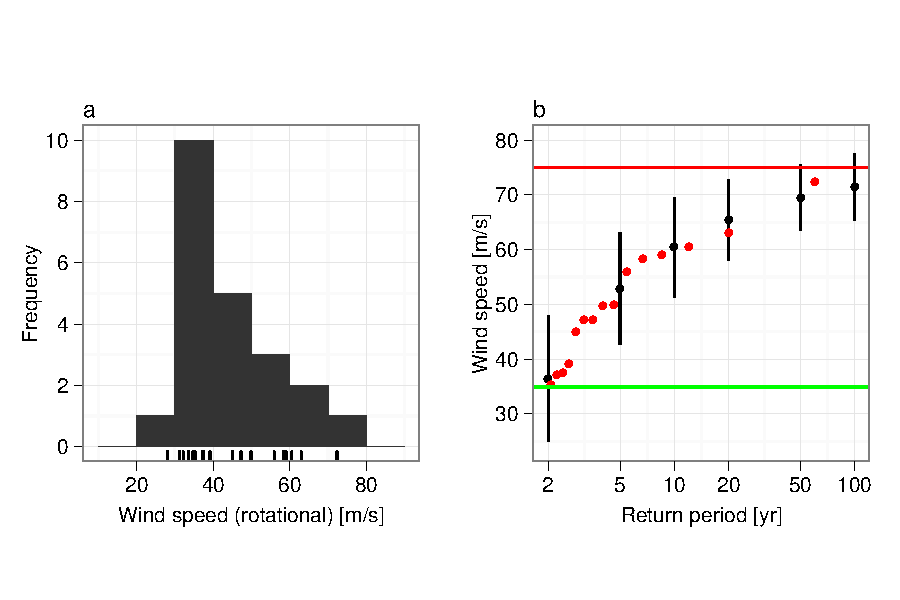
\includegraphics[scale=.65]{figures/LimitingIntensity0.pdf}
\end{center}
\vspace{-.75cm}
\alert{Limiting intensity (LI)} is the red line in panel b: A statistical estimate that we can use to compare with theoretical MPI. How should we make this comparison? Absolute values of LI are not as important as how LI changes with ocean temperature (SST). How do we estimate how LI changes with SST?
\end{frame}

\begin{frame}{Data}
Hurricanes travel over seas having varying temperature. So we need to match SST with hurricane intensity.
\begin{center}
\vspace{-3.25cm}
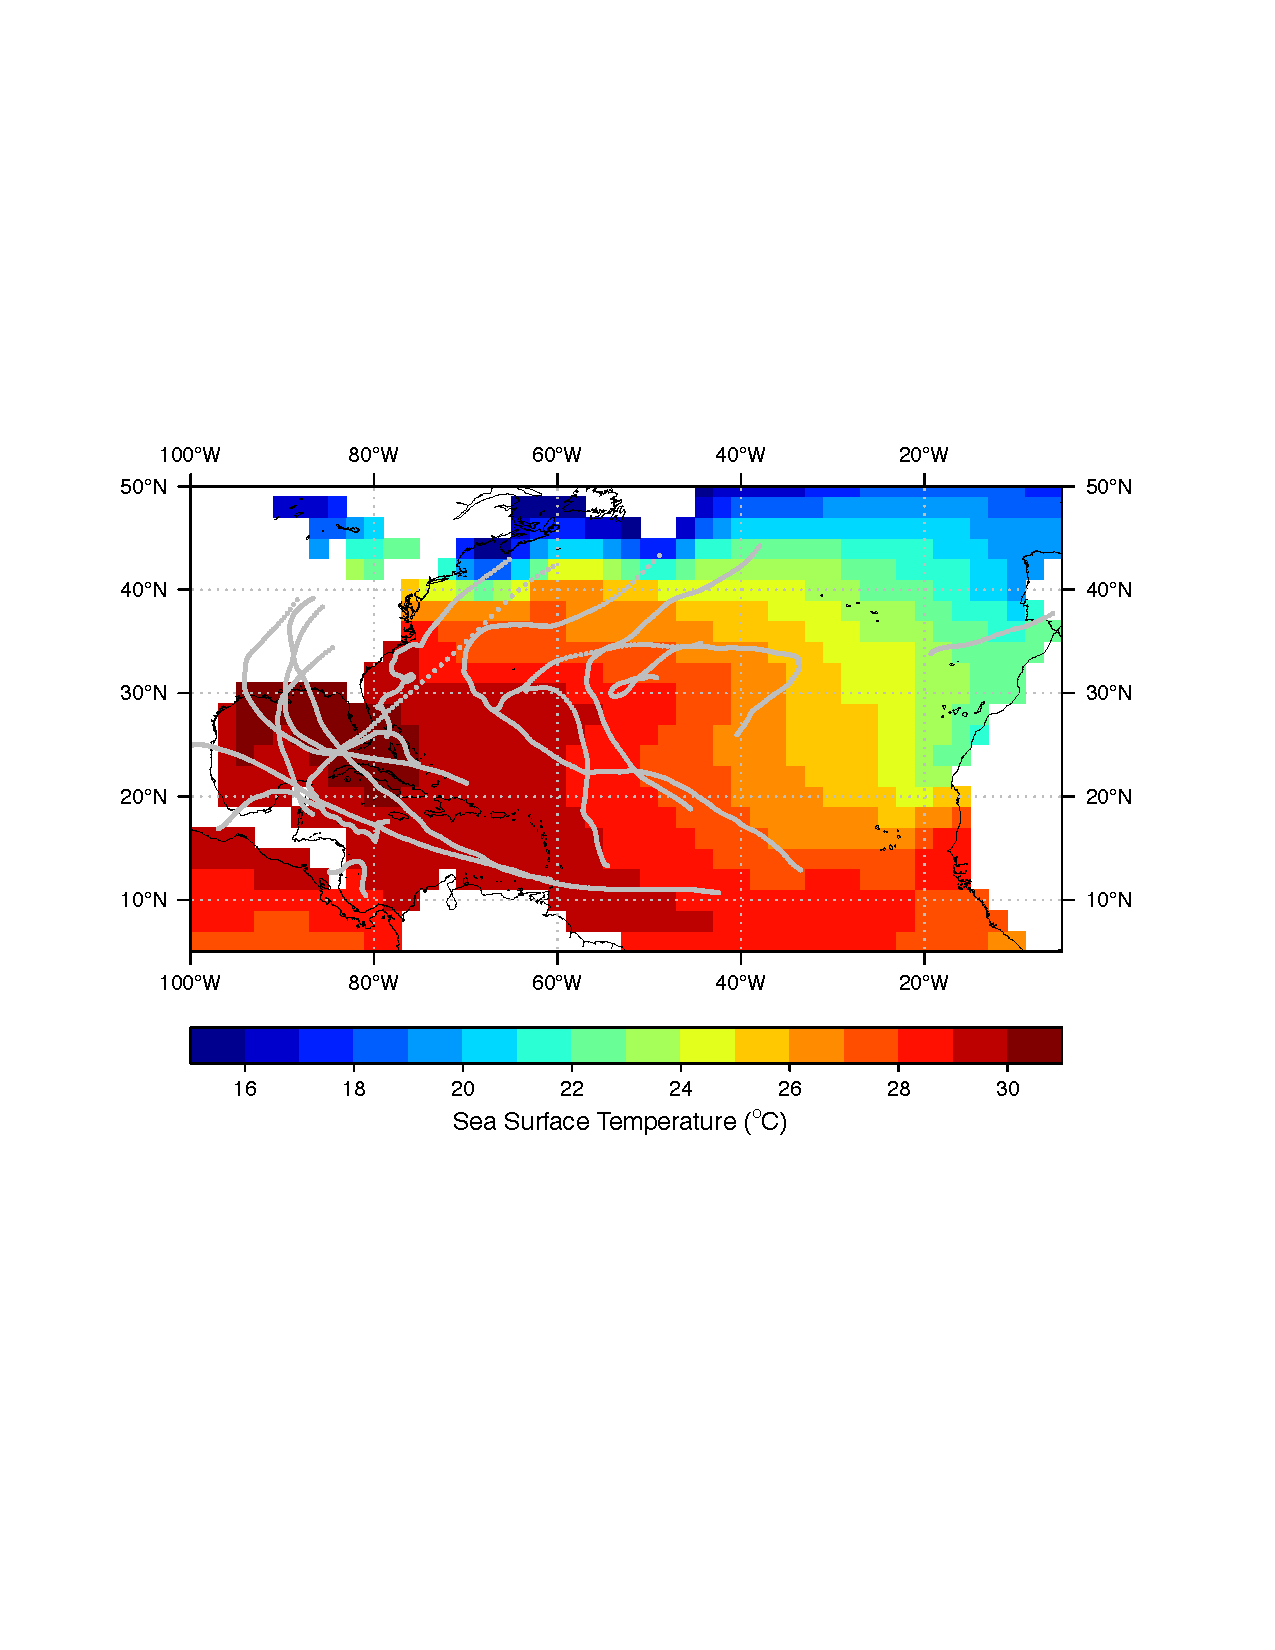
\includegraphics[scale=.5]{figures/TracksSST.pdf}\\
\end{center}
\end{frame}

\begin{frame}{Grid cells}
We collect information about each hurricane as it passes through each cell. The cells only cover  areas where hurricanes occur. Hexagons efficiently tile the region.
\vspace{-.5cm}
\begin{center}
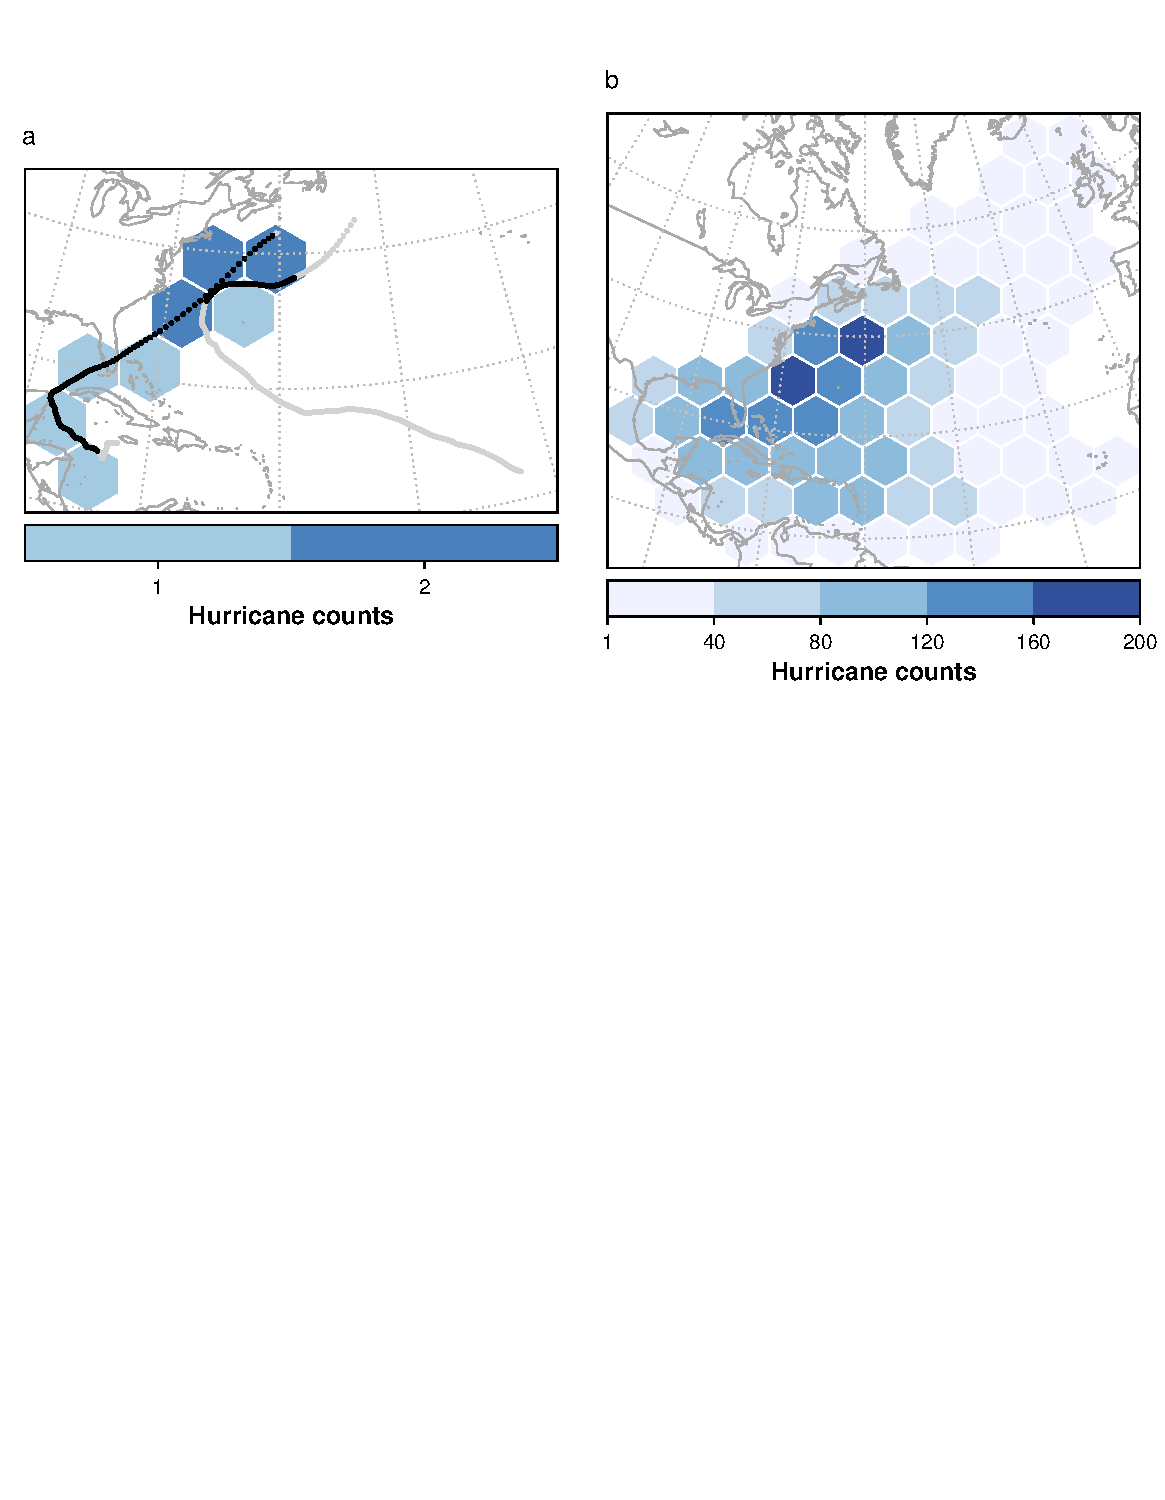
\includegraphics[scale=.51]{figures/TracksToGrids00.pdf}\\
\end{center}
\end{frame}

\begin{frame}
\begin{center}
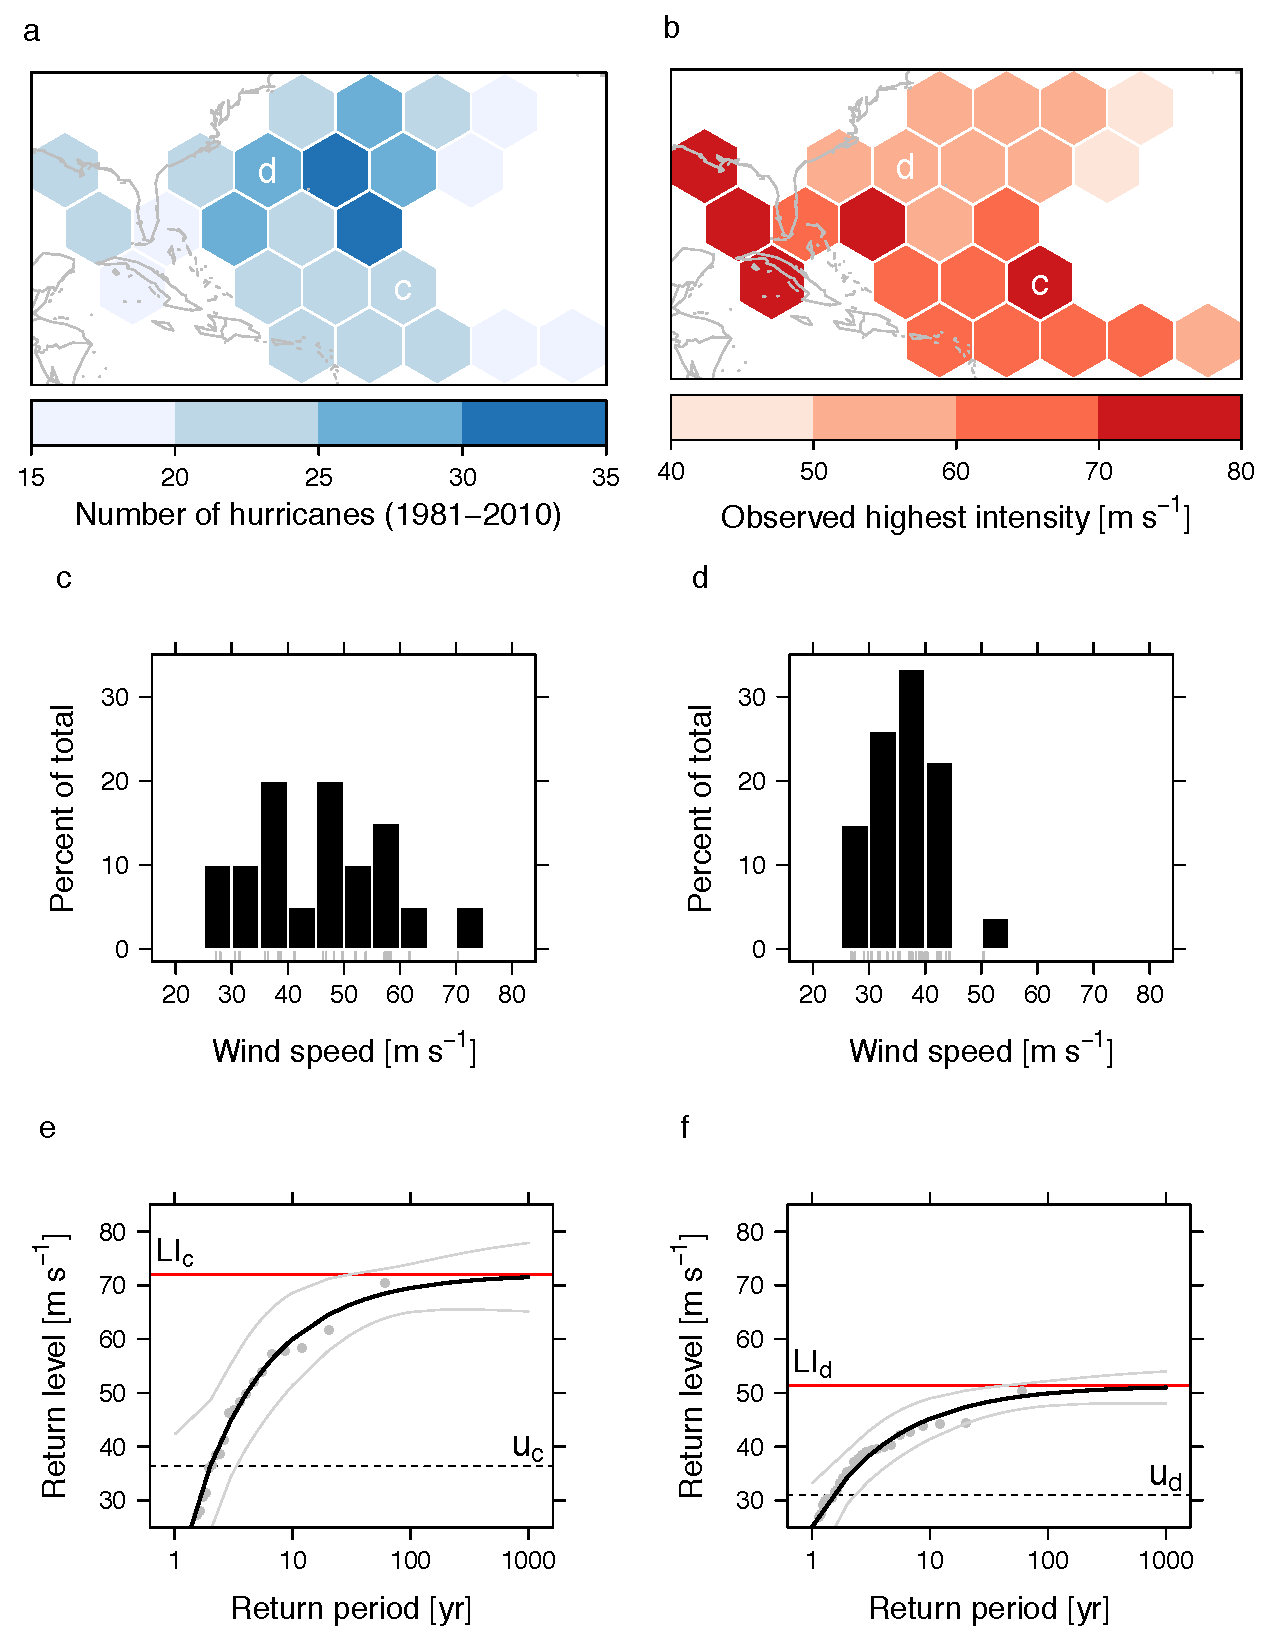
\includegraphics[scale=.3]{figures/LimitingIntensity.pdf}
\end{center}
\end{frame}

\begin{frame}{Sea surface temperature (SST) \& limiting intensity (LI)}
\begin{center}
\includegraphics[scale=.32]{figures/SSTvsLI.pdf}
\end{center}
\end{frame}

\begin{frame}
\begin{center}
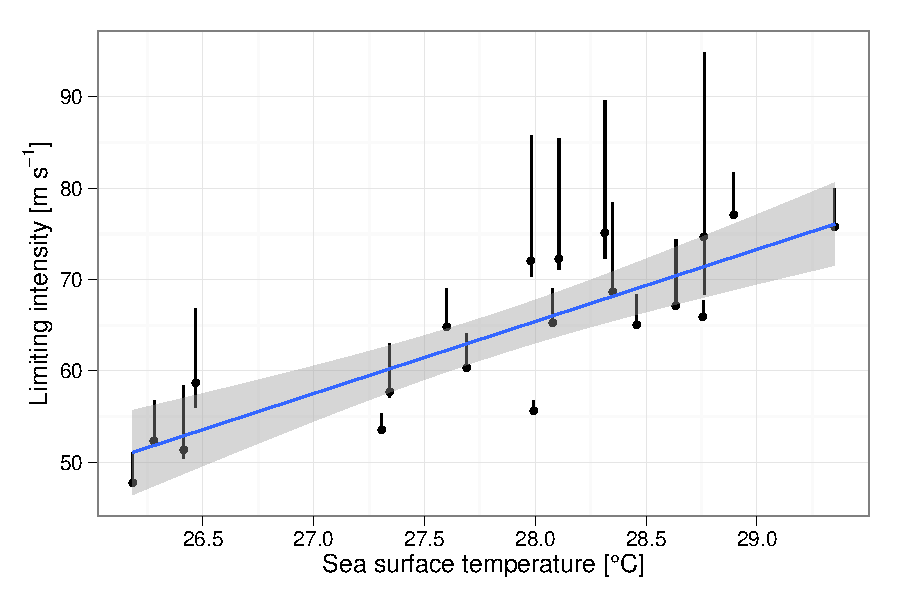
\includegraphics[scale=.65]{figures/Sensitivity.pdf}\\
We estimate the sensitivity to be \alert{8 $\pm$ 1.2 m~s$^{-1}$ K$^{-1}$ (s.e.)} for hurricanes over seas hotter than 25$^\circ$C.
\end{center}
\end{frame}

\begin{frame}{Observed vs climate model sensitivity}
\begin{center}
Observed sensitivity (left) = 8 m~s$^{-1}$ K$^{-1}$\\
HiRAM sensitivity = 2 m~s$^{-1}$ K$^{-1}$\\
\vspace{-1cm}
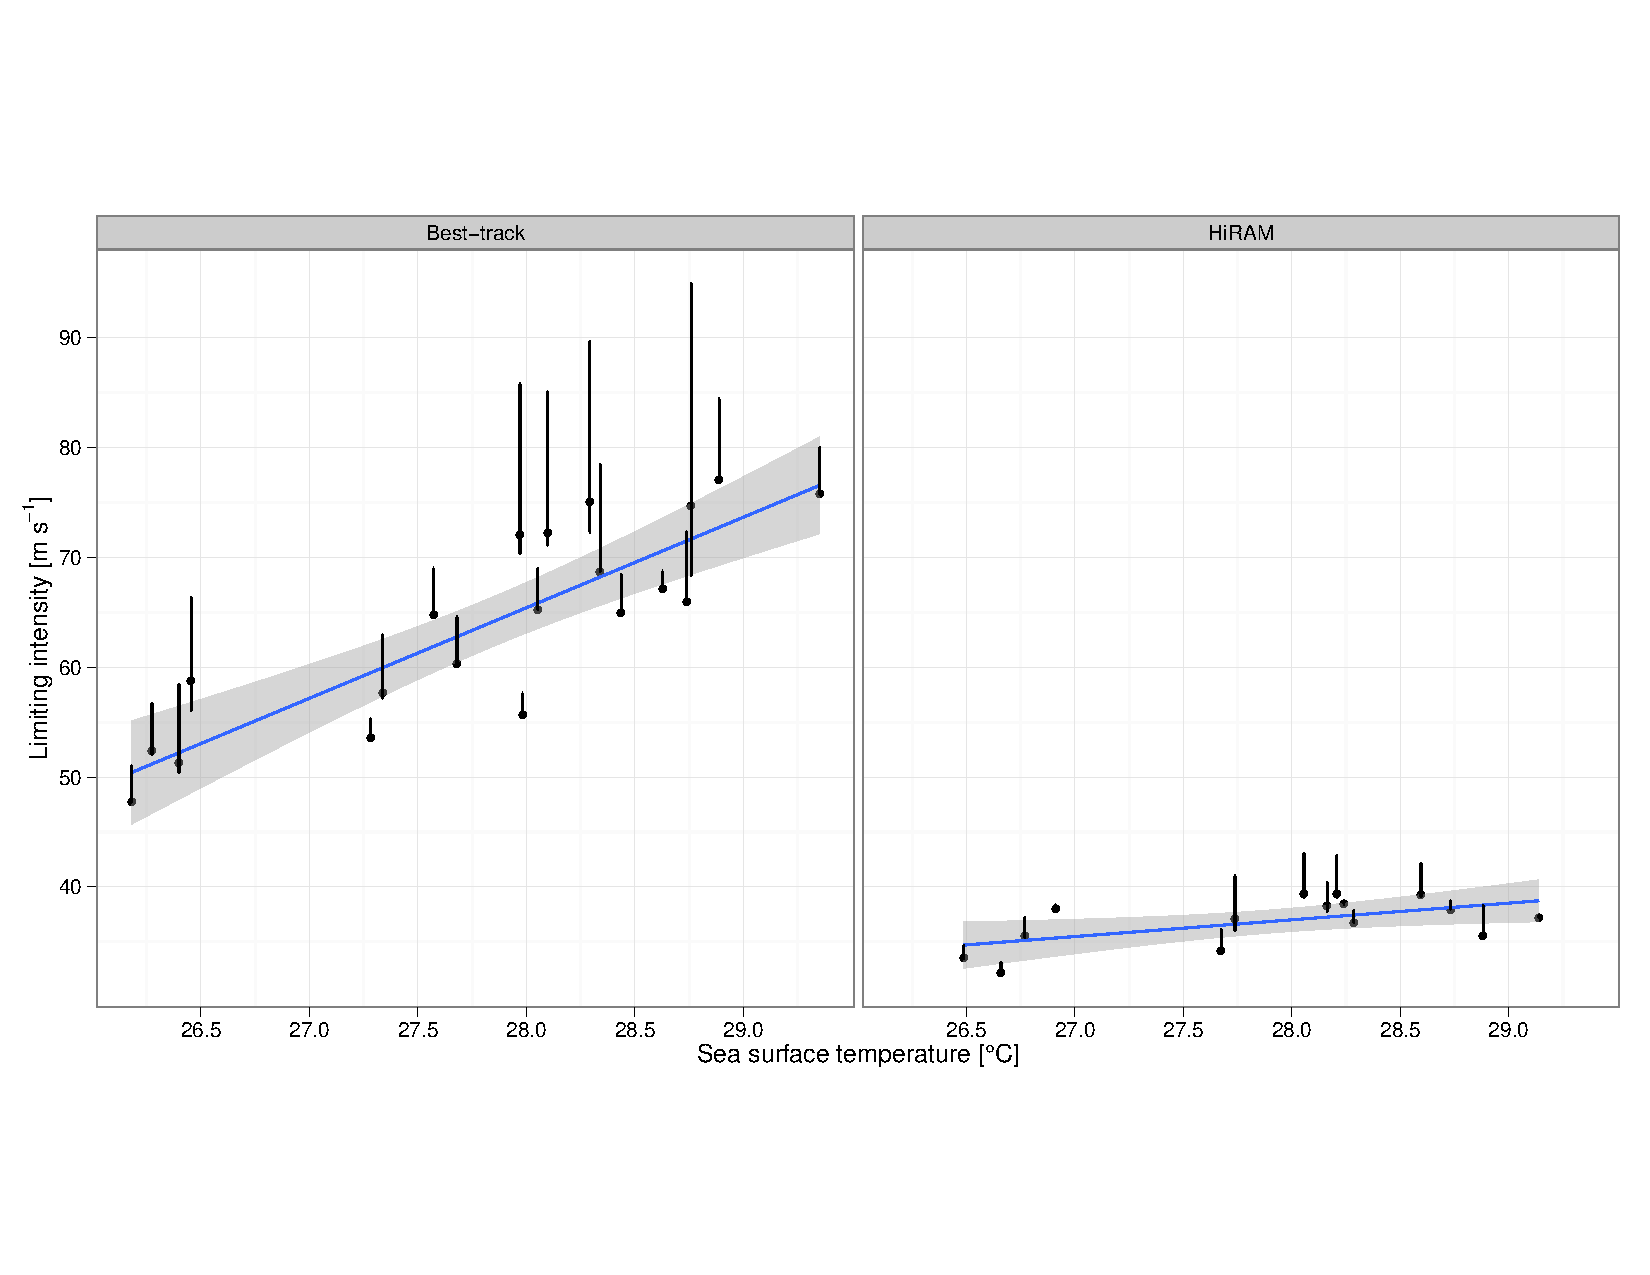
\includegraphics[scale=.37]{figures/sensHiRAMPlusOBS.pdf}\\
\end{center}
\end{frame}

\begin{frame}{Observed vs climate model sensitivity}
\begin{center}
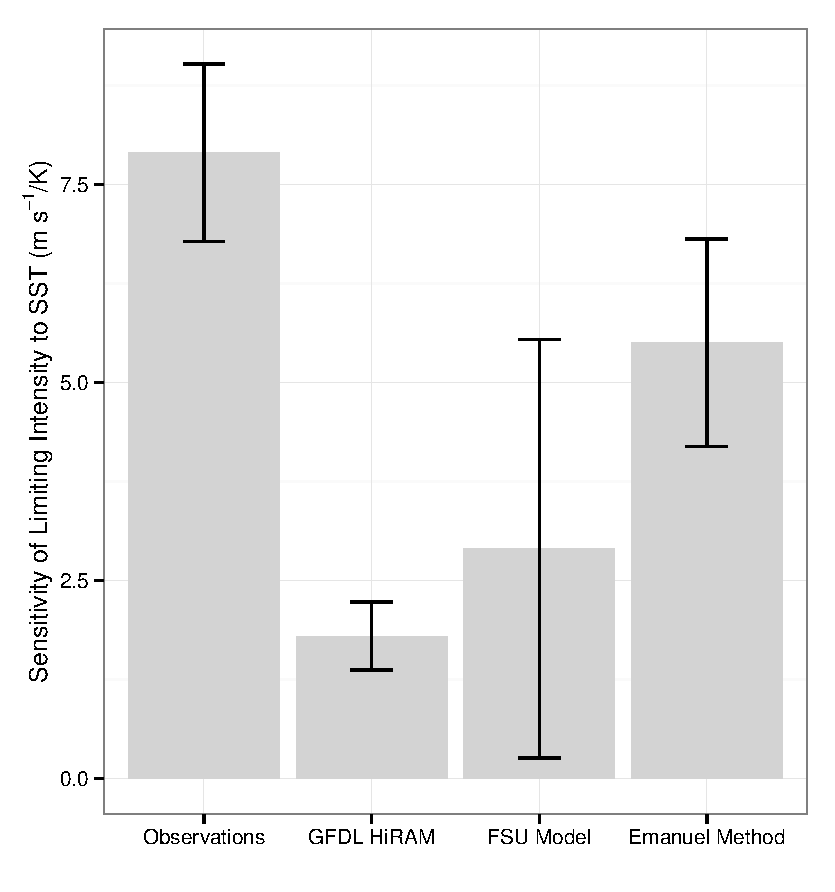
\includegraphics[scale=.5]{figures/BarPlotSensitivity.pdf}\\
\end{center}
\end{frame}

\begin{frame}{Why is this important?}
\begin{center}
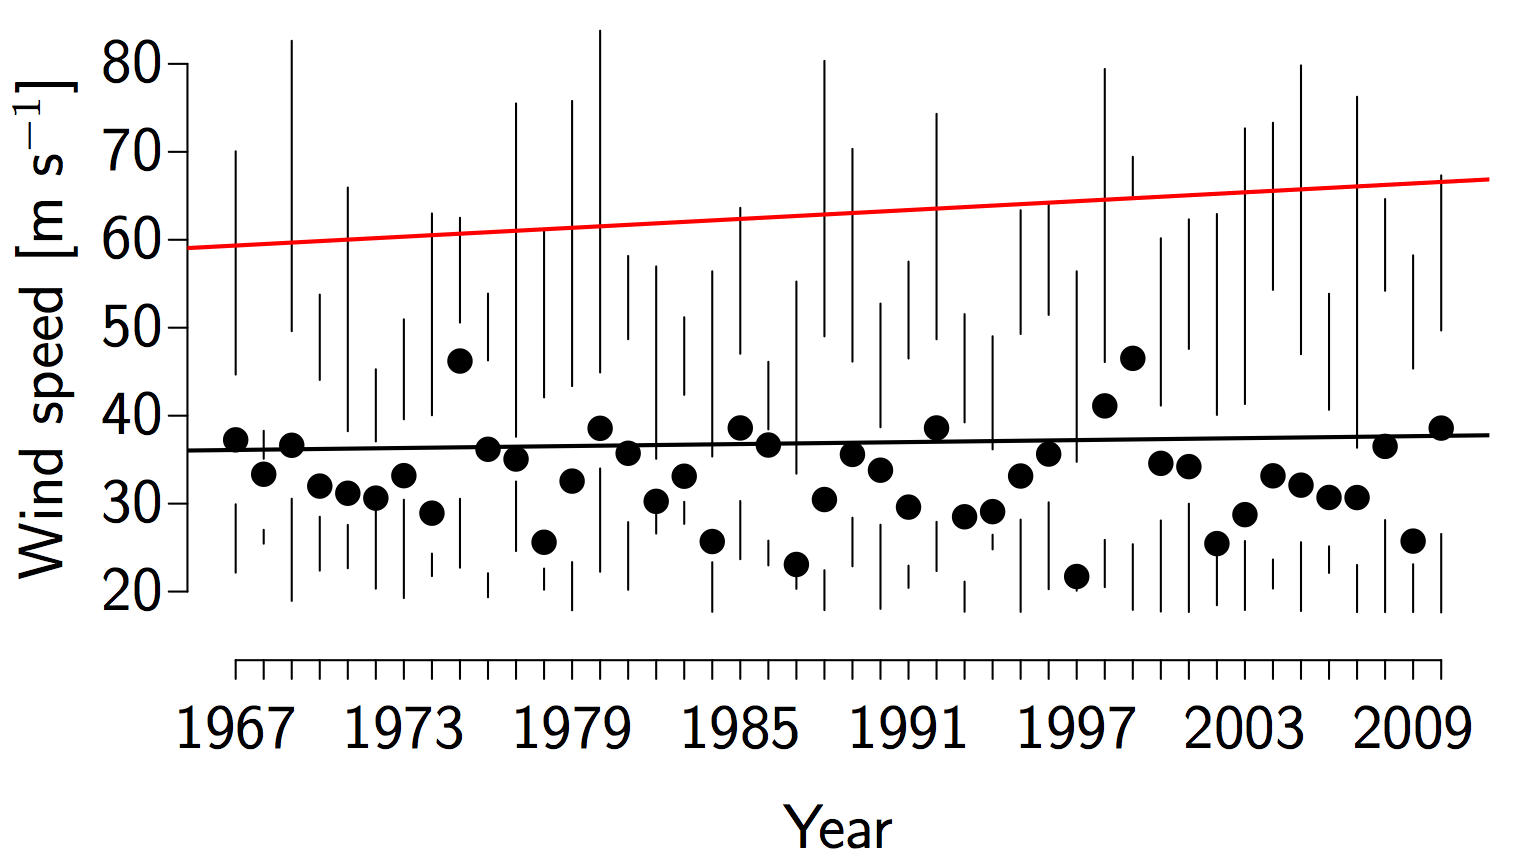
\includegraphics[scale=.18]{figures/TimeSeriesLMI.png}\\
The strongest hurricanes are getting stronger at a rate of\\ 1 m~s$^{-1}$/decade.
\end{center}
\end{frame}

\begin{frame}
\begin{center}
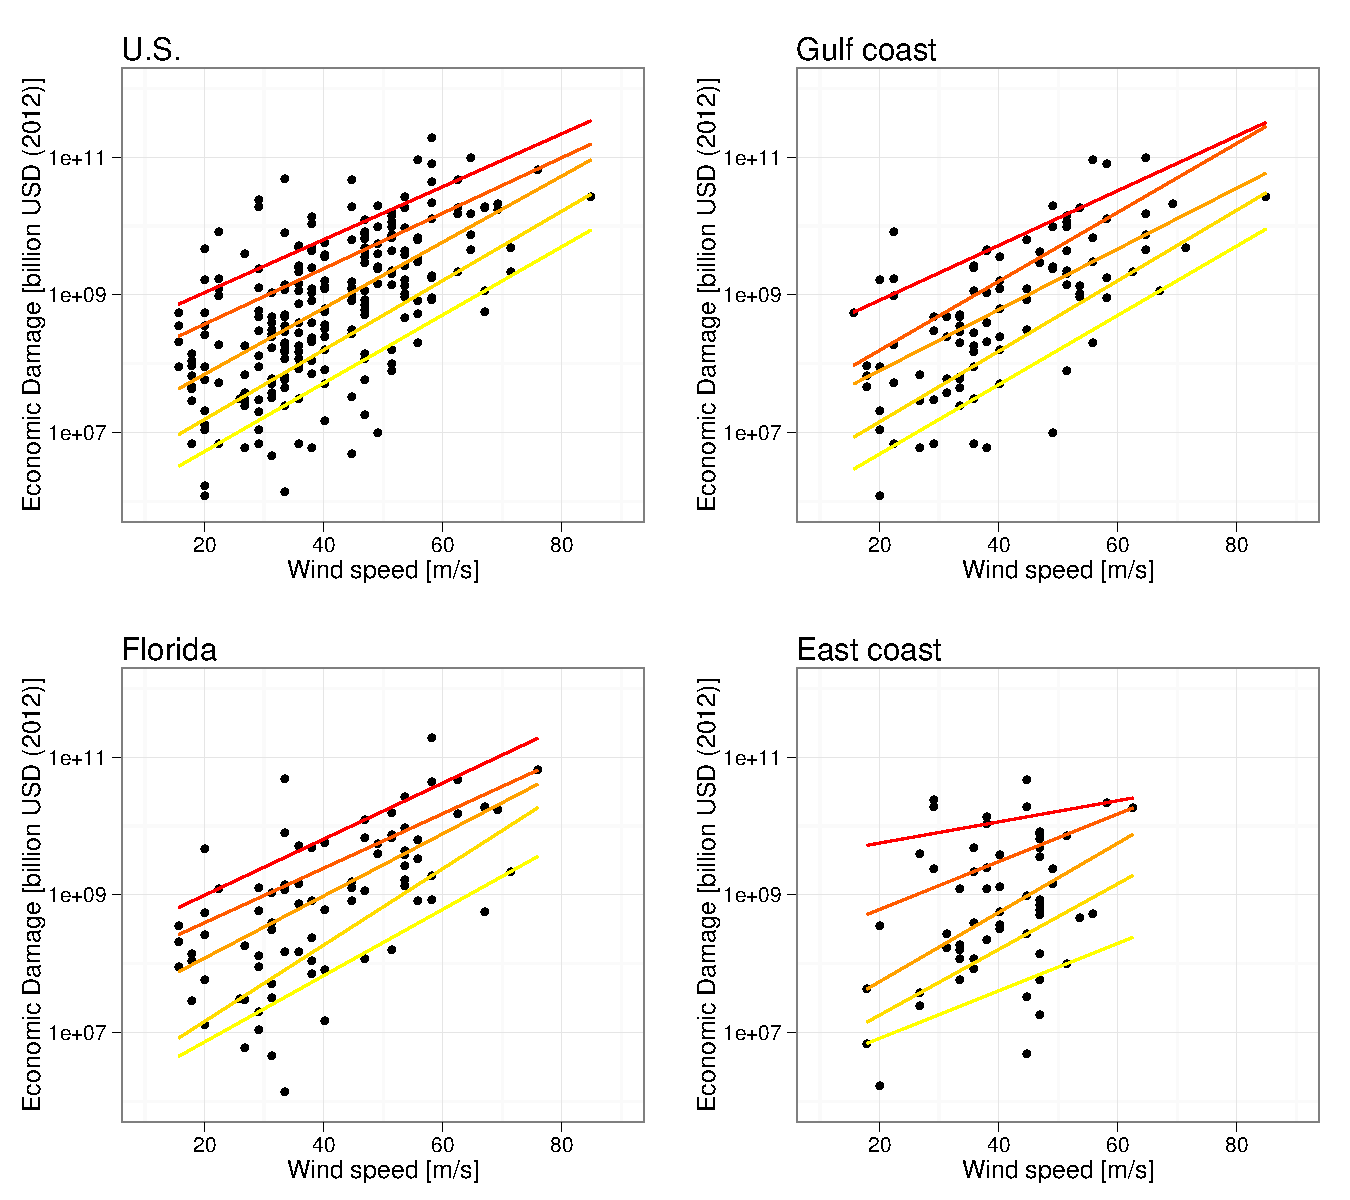
\includegraphics[scale=.35]{figures/DamageLoss.pdf}\\
Losses increase by 5\% per 1 m~s$^{-1}$ increase in wind speed.
\end{center}
\end{frame}

\begin{frame}
\huge{Thank you}\\
\huge{Questions?}\\

\large{\url{myweb.fsu.edu/jelsner/StateTornadoModel.html}}

\end{frame}

\end{document}